\documentclass{report}
\usepackage[style=numeric]{biblatex}
\usepackage{multirow}
\usepackage{graphicx}
\usepackage{cleveref}

\addbibresource{references.bib}
\graphicspath{ {../assets/} }

\def\frontmatter{%
    \pagenumbering{roman}
    \setcounter{page}{1}
    \renewcommand{\thesection}{\Roman{section}}
}%

\def\mainmatter{%
    \pagenumbering{arabic}
    \setcounter{page}{1}
    \setcounter{section}{0}
    \renewcommand{\thesection}{\thechapter.\arabic{section}}
}%

\def\backmatter{%
    \setcounter{section}{0}
    \renewcommand{\thesection}{\Alph{section}}
}%

\title{Progress Report 1 \\ Serving AI applications using a distributed architecture}
\author{Waqas Ali\\{\small Supervisor: Dr. Heming Cui}\\{\small Mentor: Shixiong Zhao}}
\date{\today}
 
\begin{document}

\maketitle

\frontmatter

\addcontentsline{toc}{chapter}{\abstractname}
\begin{abstract}
\thispagestyle{plain}

In recent years, artificial intelligence (AI) has penetrated multiple dimensions of people's daily lives by making the devices they use smarter. Learning from feedback, AI programs imitate human intelligence in terms of its learn and predict. With such widespread usage, however, users demand improved functionalities and speed, pushing developers and data scientists to make their programs smarter in the midst of industry competition. These smarter programs have to deal with more complexities, and developers consequently have to choose whether to prioritize the program's features or performance, posing a dilemma for them. This project proposes to design an AI application with a distributed architecture instead of a centralized architecture (the more common structure in the status quo) in order to improve its latency and throughput. As proof of concept, the project will specifically examine a complex stock price prediction application and the goal is to transfer it onto a distributed architecture. The project's objective is to develop tooling and foundation to automatically instantiate and compare distributed systems of a variety of specifications and scheduling algorithms. It's divided into three big milestones. Firstly, the machine learning stage where a test model has to be developed and trained. Second, modifying the model to work in a distributed manner which is next. Lastly, comparing distributed implementations which is the most crucial aspect of this project. As of now, the first milestone has been completed in which a stock price prediction service has been successfully developed, trained and deployed on a single machine.
\end{abstract}

\addcontentsline{toc}{chapter}{Acknowledgements}
\section*{Acknowledgements}
In addition to my supervisor and mentor who helped me with the technical aspects of my project, I would like to thank Ms. Mable Choi for her guidance in distilling and consolidating my work in a better way.

\setcounter{page}{2}
\tableofcontents

\newpage
\addcontentsline{toc}{chapter}{\listfigurename}
\listoffigures

\newpage
\addcontentsline{toc}{chapter}{\listtablename}
\listoftables

\newpage
\mainmatter

\chapter{Introduction}

\section{Background}
Artificial intelligence is an area of computer science that focuses on granting machines the ability to act intelligently \cite{McCarthy2007}. It's a vast field with limitless applications and each application has its own unique solution. Machine learning, specifically, is a subset of artificial intelligence that learns from data. \cite{Mitchell1997} Nowadays we see ubiquitous applications of artificial intelligence such as spam filters \cite{Androutsopoulos2000},  recommendations \cite{lekakos2008hybrid}, virtual assistants and self-driving.

Customers are demanding smarter and smarter capabilities in their machines, and this trend leads to a new set of software development challenges for AI developers. \textit{Nvidia} summarises them with the PLASTER \cite{Teich2018} framework:
\begin{itemize}
  \item Programmability
  \item Latency
  \item Accuracy
  \item Size of Model
  \item Throughput
  \item Energy Efficiency
  \item Rate of Learning
\end{itemize}

These aforementioned challenges carry over to the realm of machine learning, since it is a subset of artificial intelligence. A machine learning application has two main stages:
\begin{enumerate}
  \item Training (Learning from data)
  \item Inference (Given an input, predicting an output)
\end{enumerate}

Take the example of an application that relies on a machine learning model to transcribe voice. Before the model can be used by the application, it needs to be trained. To do this, developers expose the model to hundreds of voice recordings to allow it to learn which sounds match to which words. Now, the application can use the model by sending it voice recordings and receiving transcribed text in return. In short, this process of predicting an output in response to an unseen input is inference, the second stage of machine learning as mentioned previously.

\section{Motivation}

\begin{figure}
  \centering
  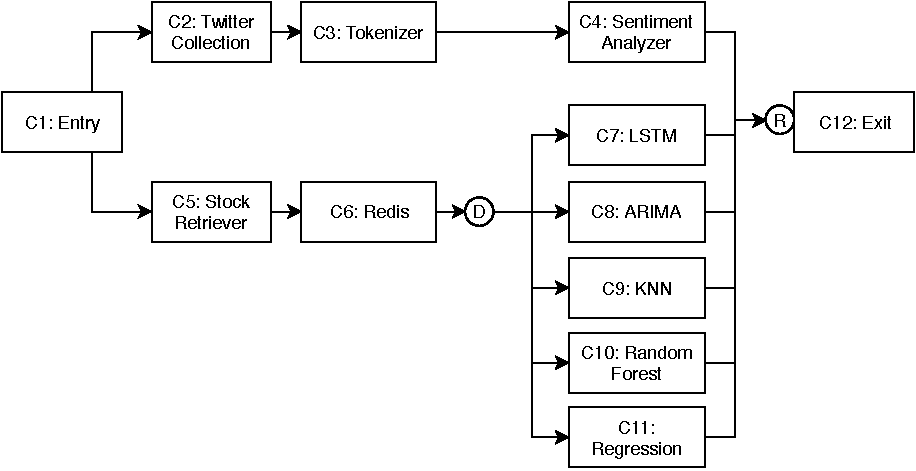
\includegraphics[width=\textwidth]{StockPriceServiceBasic.pdf}
  \caption{Inference pipeline of a basic stock price prediction service. C2 and C5 are data retrievers which fetch past stock data and twitter mentions of a specified stock symbol. C6 is a caching layer which allows skipping C7-C11 steps if a prediction has been recently made for a specific stock symbol. C7, C8, C9, C10 \& C11 are ML models that compete against each other to predict a stock symbol's price. C4 is a sentiment analyzer whose results are taken into account for price prediction. As can be seen, it's a fairly complex pipeline composed of several different steps.}
  \label{fig:StockPriceServiceBasic}
\end{figure}

Since end-users of machine learning applications are only concerned with inference, not training, inference must be quick.

For inference, an input goes through multiple steps, known as a pipeline. Figure \ref{fig:StockPriceServiceBasic} is an example of a stock price prediction service's pipeline. As tasks in a pipeline increase in quantity and complexity, it can increase the \textit{latency} (time taken) to execute all steps of the pipeline. Moreover, if a \textit{centralized architecture} (single machine) executes the complete pipeline, it can create bottlenecks. For example, if a pipeline for input A is in progress, the pipeline for input B cannot start.

On a centralized architecture, all tasks have to be done sequentially (even if they are independent of each other). This could take a long time and hence increase the latency. Moreover until all tasks for a specific request have finished, processing for a new request cannot start. Thus, the service cannot handle a high number of requests in a given period i.e. \textit{throughput}.

\section{Contribution}

Several methods could be considered to optimize the latency and throughput of an artificial intelligence application.

This project attempts to tackle this optimization problem by efficiently distributing the pipeline tasks over several machines. The claim is that, theoretically, we can improve the latency and throughput of an AI application (concerns which were highlighted in the PLASTER framework \cite{Teich2018}) if decentralized architecture is employed instead of centralized architecture.

\section{Objectives}\label{objectives}

There are two steps to developing any distributed application:
\begin{enumerate}
  \item Program the application in a way as to take advantage of multiple machines.
  \item Deploy the application on a network of machines.
\end{enumerate}

Therefore, moving an artificial intelligence application from a centralized architecture to a distributed network not only requires deploying it on a network of multiple machines but modifying it to utilize the newly available resources.

Since every application is unique, devising a general technical solution for accomplishing the above two steps will be infeasible. Therefore, the project will choose one AI application as a proof of concept and use that as a testing ground of the solution proposed in previous section.

A distributed application's success depends on how the application divides its tasks (job scheduling) and quality/quantity of resources available for use. To figure out what works best we need a quick and reliable way of testing different job scheduling algorithms on networks of different sizes composed of machines of different specifications.

Consequently, the project's objectives are to develop the following programs:
\begin{enumerate}
  \item An AI application with a complex inference pipeline which can accept different job scheduling algorithms.
  \item A deployment script that can programmatically buy cloud resources and deploy our AI application according to provided specifications.
  \item A web app to measure latency and throughput.
\end{enumerate}

Given the above objectives are fulfilled, we can confidently argue for or against using distributed systems for AI applications.

\section{Report Organization}
The remainder of this report is organized as follows. \Cref{chap:methodology} describes and justifies the methodology. \Cref{chap:schedule} breaks the project into milestones and gives a schedule with estimated completion time for each. Following this, \cref{chap:progress} reports current progress and \cref{chap:limitations} discusses limitations and difficulties faced so far. Lastly, \cref{chap:conclusion} summarises lessons learned and future steps.

\chapter{Methodology}\label{chap:methodology}

\section{Choose AI Application for testing}
As the project proposes a distributed architecture for artificial intelligence applications in general, our test AI application must be a sufficient representative of most if not all AI applications for a fair investigation. Naturally, a fairly representative application is one with a pipeline composed of different kinds of tasks with a mix of mutually dependent and independent ones. Ergo, choosing a single AI application as a testing ground for our solution is an important task that requires studying popular AI techniques and implementations in the community.

\section{Develop basic model}
Every AI or ML application starts with data science. First of all, a machine learning model needs to be trained and an inference pipeline needs to be developed. This requires studying current techniques for the application of our choice and using that knowledge to build and train a good enough model. At this stage, accuracy isn't important so we don't need to fine-tune the model. Once the model training is done, it needs to be ready for inference. Therefore, we need to ensure that all the steps required to accomplish inference on a new unseen input have been implemented at a satisfactory level.

\section{Run on a centralized system}
By now we have chosen a test AI application and trained a basic model for it. Moving on, we need to ensure we can successfully run inference on a single machine on the cloud. This step is important for two reasons. Firstly, this gives us a baseline performance we can compare our distributed implementations with. Second, we will have a working implementation of our application and we can refer to it while converting our application to a distributed implementation.

\section{Convert to a distributed system}
Consequently, the next step is to convert the application from a centralized implementation to a distributed implementation. This will require modifying the source code to use distributed system techniques such as RPC (remote procedure call). To ensure consistency, we should ensure our distributed implementation running on one machine has the same performance as the centralized implementation of earlier.

\section{Programmatic Deployment}
The only way to test a distributed implementation is to deploy it on a network of computers and measure performance. Cloud services make it considerably easy to do so without having to deal with actual hardware. After this stage, we should be able to automatically instantiate cloud resources according to provided specifications and deploy the distributed implementation of our application on them. We can also deploy our implementation on the cloud manually but that will take a lot of time and considering the number of times we would have to do it, it isn't feasible. Besides, we need to ensure all implementations are reproducible and consistent. 

\section{Compare}
With all these different implementations, we need a reliable way of comparing each implementation's performance that is completely decoupled from its intrinsic qualities. A fair and reliable way to compare is to create a web app that accepts a server URL and sends numerous requests to it. Consequently, it measures latency for each request and throughput in general. As the web app is run in the browser, it measures these metrics from the client-side and all it cares about is input and output. Thus, it does not matter for the web app if the server implementation is on a centralized or distributed architecture as long it receives an output.

\subsection{Test Cases}
To study whether a distributed architecture can indeed improve latency and throughput, performance will be compared across systems of various specifications:
\begin{enumerate}
  \item Centralized implementation (baseline)
  \item 1 machine for n tasks (should be same as above)
  \item Less than n machines for n tasks
  \item n machines for n tasks (optimum)
\end{enumerate}

\chapter{Schedule}\label{chap:schedule}
To accomplish the objectives in section \ref{objectives}, the project follows the following schedule. It's composed of milestones with a target completion month for each.
\begin{table}[h!]
  \begin{center}
    \caption{Project Schedule}
    \label{tab:table1}
    \begin{tabular}{ |l|l| } 
      \hline
      \multicolumn{2}{|c|}{2019} \\ \hline
      \multirow{3}{*}{October} & Choose \& Design AI application to work on \\
       & Develop a basic inference pipeline on a centralized architecture \\
       & Progress Report 1 \\ \hline
      \multirow{3}{*}{November} & Convert pipeline to work on a distributed system using RPC \\
       & Web app to measure latency and throughput \\
       & Progress Report 2 \\ \hline
      December & Manually deploy pipeline to distributed architecture on cloud \\ \hline
      \multicolumn{2}{|c|}{2020} \\ \hline
      \multirow{3}{*}{January} & Programmatically instantiate cloud resources and deploy model \\
       & First Presentation \\
       & Detailed interim report \\ \hline
      February     & Vary deployments by cloud resources and measure latency/throughput on each  \\ \hline
      March     & Enhance AI inference pipeline by adding more steps  \\ \hline
      \multirow{3}{*}{April} & Finalize implementation \\
       & Final Presentation \\
       & Final Report \\ \hline
      \end{tabular}
  \end{center}
\end{table}

\chapter{Progress}\label{chap:progress}

\begin{figure}
  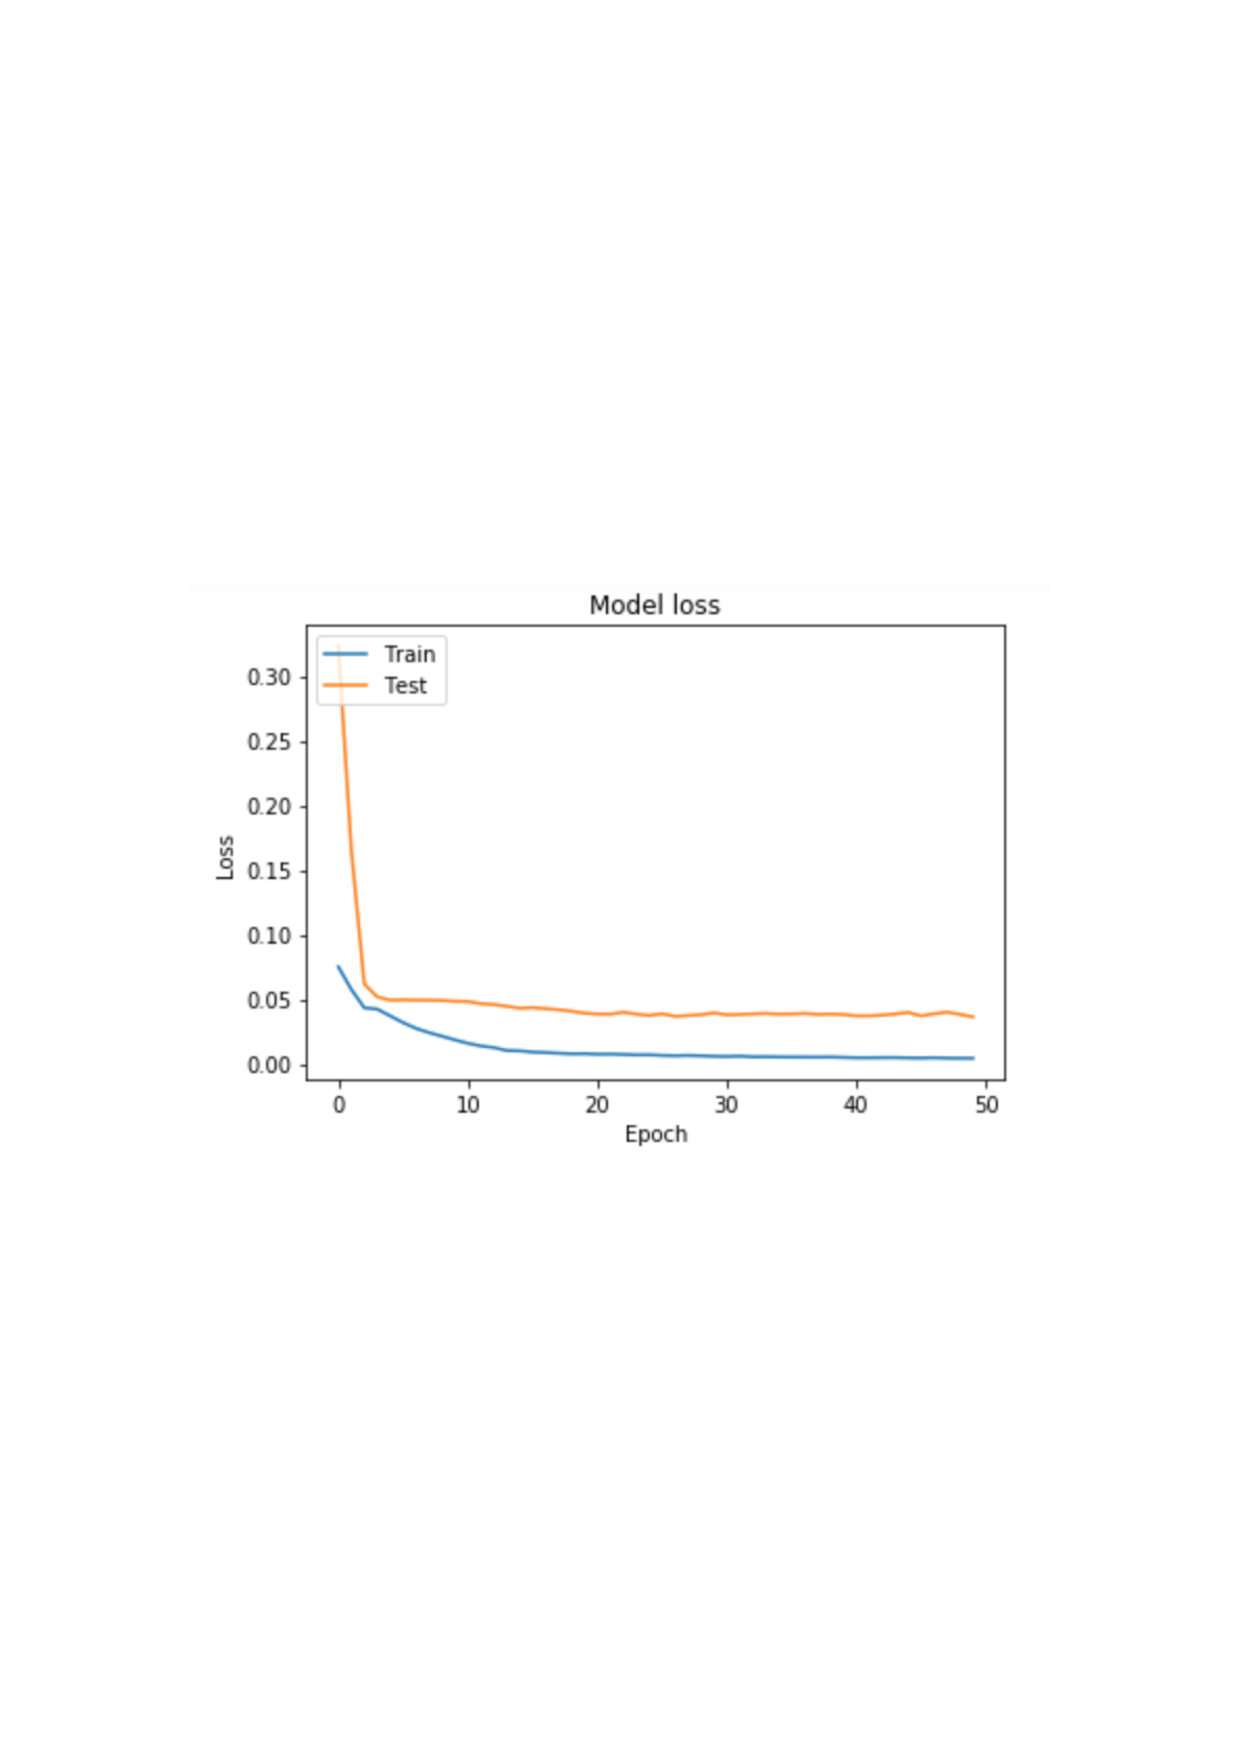
\includegraphics[width=\textwidth]{EpochVModelLoss.pdf}
  \caption{This graph shows how our model learned from GE's historical stock price data. An Epoch means a round of training and Loss means how far off we are from actual values. A lower loss means a more accurate data. Train means the performance of our model on training data (data it uses to train itself). Test means the performance of our model on testing data (data it only uses for measuring performance and does not use to train itself at all). As can be seen, our model trains well quickly as the loss drops rapidly after 5 rounds.}
  \label{fig:EpochVModelLoss}
\end{figure}

\section{Summary}
As of now, the first three milestones mentioned in \Cref{chap:methodology} are finished. I have chosen an AI model, developed a basic model, ran inference successfully on a single machine and built a latency measuring web app.

\section{Stock Price Prediction}
\subsection{Why?}

After consultation with my mentor and careful research, I chose stock price prediction as my AI application. Input any stock symbol and it will predict its price on the next day. There are many ways to make such a prediction. One approach is to analyze past prices and predict the stock price behavior based on that. However, this approach completely ignores the market and current affairs. An interesting approach would be to use cutting edge time series forecasting models combined with sentiment analyzers to combine the best of both worlds.

\subsection{Challenges}

\begin{figure}
  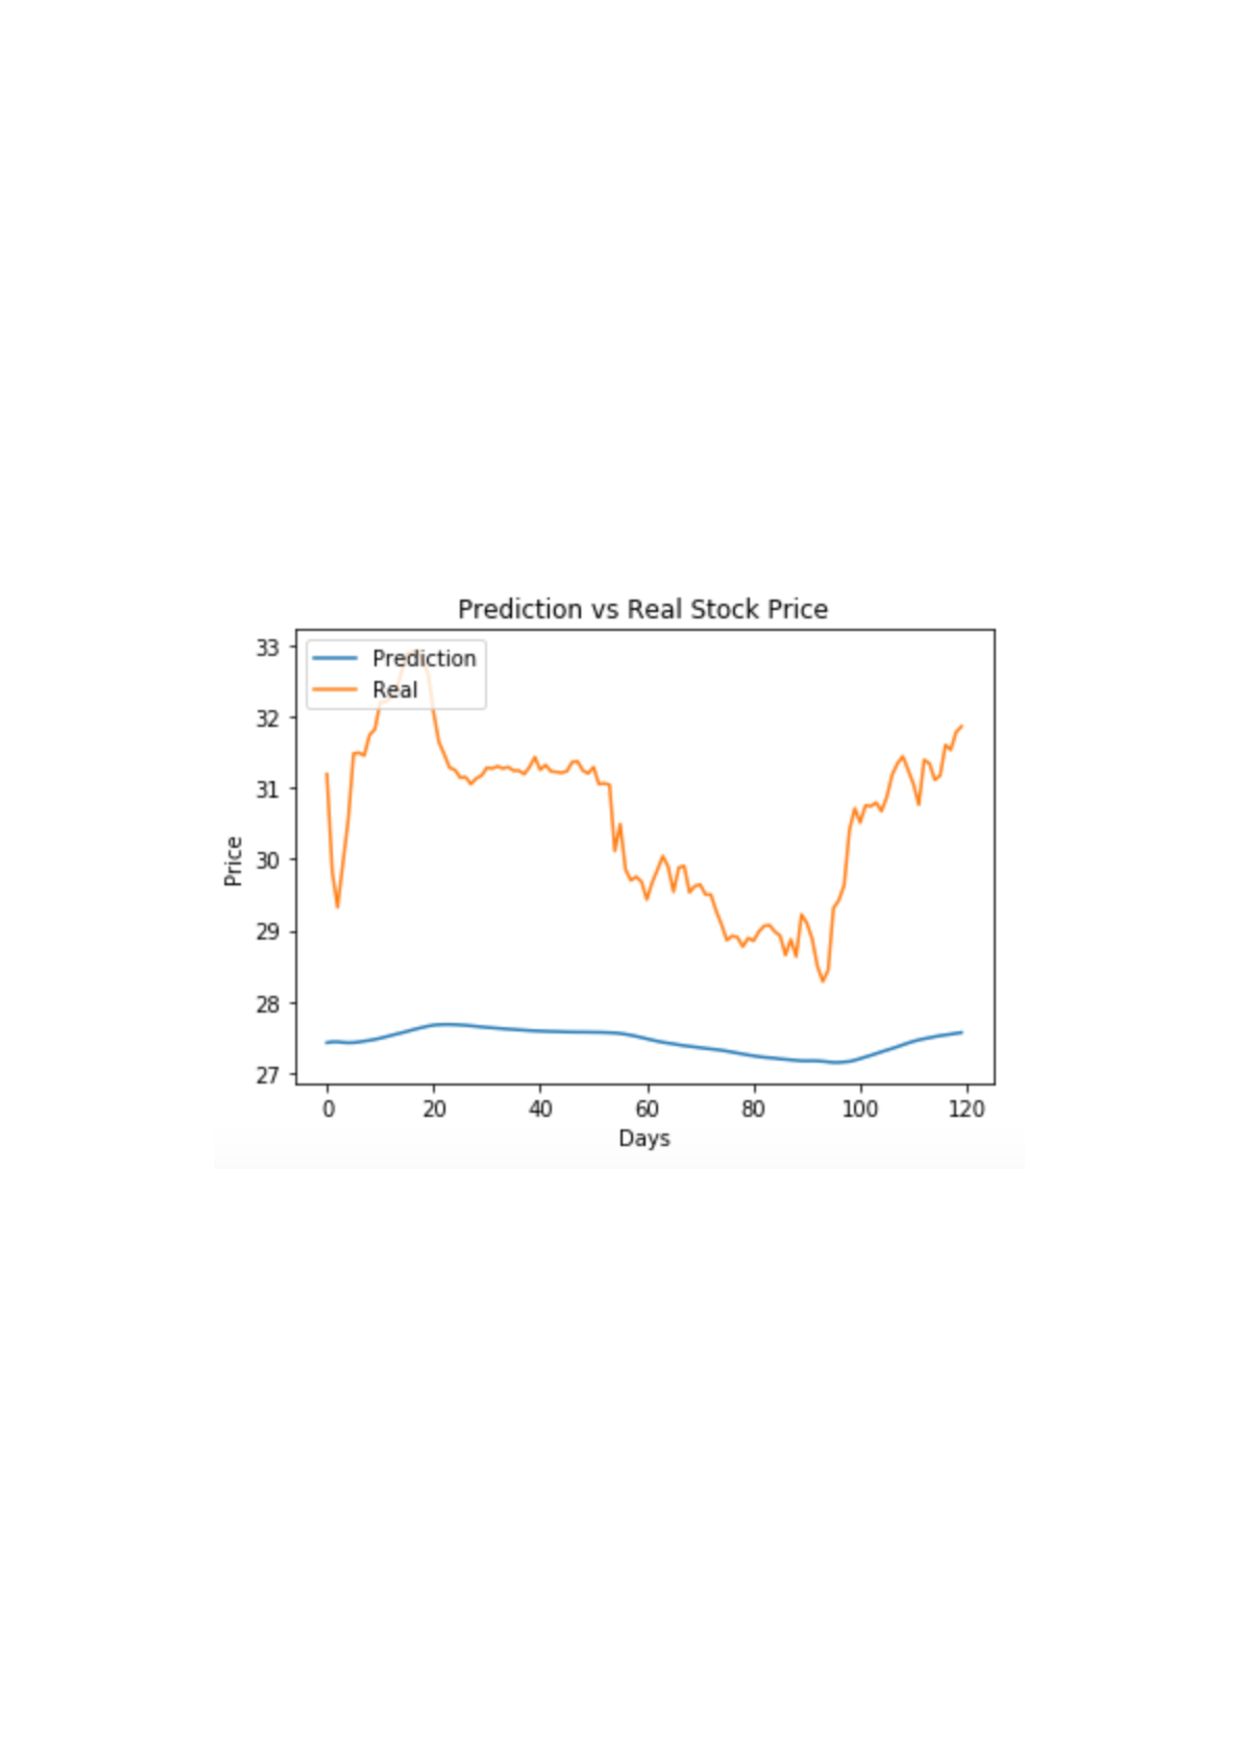
\includegraphics[width=\textwidth]{PredictionRealPrice.pdf}
  \caption{This graph shows our model's predicted price for GE's stock for 120 days and the actual price for those 120 days. As can be seen, our model can do better but it captures the direction of the trend well. Predicted price and real price both show increase around the 20th day and both show a drop around the 90th day.}
  \label{fig:PredictionRealPrice}
\end{figure}

As the stock price prediction service should be able to predict prices for any number of the thousands of stock symbols out there and there is always something new happening in the context of current affairs, it is infeasible to train the model in advance for all stock symbols. Therefore, whenever the service is tasked with predicting price for a stock symbol it has to retrain itself and then carry out inference. All in all, this process of training and then inference creates huge latency. As can be seen in Figure \ref{fig:StockPriceServiceBasic}, there are a lot of tasks that can be done independently. Hence, stock price prediction service is a prime testing ground for application of distributed computing in artificial intelligence.

\section{Deployment on a single machine}

As a baseline, I took the machine learning model I just developed and deployed it onto a single machine ready for inference.

\section{Web app for measuring metrics}

In addition I have setup a basic web app that accepts the server URL above and measures the latency for stock price prediction. I haven't added throughput measurement yet.

\chapter{Limitations and Difficulties}\label{chap:limitations}
\section{Personal Limitations}
As I don't have enough experience working with time series data, a lot of my time has been spent on learning how to properly develop a machine learning model for it. Moreover, I have had to learn a lot of time series forecasting techniques mentioned in Figure \ref{fig:StockPriceServiceBasic} which has taken considerable time.

\section{Potential Difficulties}
I have never implemented a distributed architecture using python and I can already foresee me having to learn how to do that for my next step. Moreover, the current baseline model takes a long time to train and I am not sure whether I can bring down the time enough even if I use a distributed architecture. Lastly, I will need a cloud service account where I can instantiate required resources. Based on previous experience, it is not the most straightforward process. So I will have to figure out how I can do that.

\chapter{Conclusion}\label{chap:conclusion}
As of now, I am on track as far as the schedule is concerned. I have a foundation to build upon and next steps are to convert the stock price prediction service into a distributed architecture. However, as I have only tackled the machine learning aspect of my project until now and I have yet to dive into the distributed system aspect, I am uncertain of how difficult it will be. 

\backmatter

\addcontentsline{toc}{chapter}{Bibliography}
\printbibliography

\end{document}